%
%=============================--C--=============================%
\clearpage
\subsection{3. Desmodulaç\~ao}
No que consta à desmodulação, o processo é efetuado em dois instantes: sincronização de símbolo (efetuada no bloco \textit{Symbol Sync}) e reconversão para stream de dados binários (\textit{Binary Slicer}).

\subsubsection{3.1 \textit{Symbol Sync}}
\label{subsubsec:symbol-sync}
\begin{quote}
    "Symbol timing synchronization has a unique purpose: to find the optimal instants when downsampling a sequence of samples into a series of symbols. In other words, it focuses on selecting the “best” sample out of every group of samples, such that this selected sample can better represent the transmitted symbol. The chosen sample (deemed as the symbol) is then passed on to the symbol detector."\cite{igor}
\end{quote}

\begin{figure}[H]
    \centering
    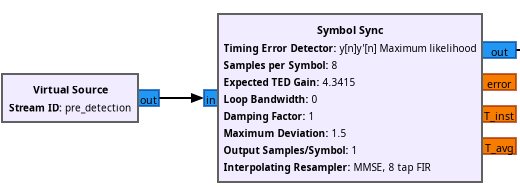
\includegraphics[width = 0.6\linewidth]{img/intro/demod1_symbolsync.png}
    \caption{Bloco que realiza a sincronização de símbolo.}
    \label{fig:symbolsync}
\end{figure}

Concentramos a nossa atenção sobre os seguintes parâmetros: 

\begin{table}[h]
    \centering
    %\setlength{\extrarowheight}{1em}
    \begin{tabular}{l l}
        \minipage[t]{0.5\linewidth-2\fboxsep-2\fboxrule\relax}
            \textbf{\textit{Loop Bandwidth:}}\newline
            "It should nominally be close to 0, but greater than 0. If unsure, start with a number around 2*pi*0.04, and experiment to find the value that works best for your situation."\cite{symbolsync-gnuradio}
        \endminipage &\
        \minipage[t]{0.5\linewidth-2\fboxsep-2\fboxrule\relax}
            \textbf{\textit{TED Gain:}}\newline
            "This value is normally computed by the user analytically or by simulation in a tool outside of GNURadio. This value must be correct for the loop filter gains to be computed properly from the desired input loop bandwidth (...)"\cite{symbolsync-gnuradio}
        \endminipage
    \end{tabular}
\end{table}
\vspace{-1.5em}
\paragraph{3.1.1 \textit{TED (Timing Error Detector)}}\mbox{}\\
\label{subsubsubsec:loopbandwidth}
Tal como supracitado, o bloco \textit{Symbol Sync} requer a computação do \textit{TED Gain} fora do ambiente \textit{GNU Radio} para um correto funcionamento face à \textit{Loop Bandwidth}.

\begin{quote}
"(...) The timing offset error $\tau$ results from the channel propagation delay, which can not be controlled and, therefore, introduces delays that are not simply integer multiples of the symbol period. In reality, the propagation delay is such that $\tau$ is composed of two terms: an integer and a fractional multiple of $T_s$. In the context of symbol timing recovery, we are only concerned with the fractional error. The integer error is handled by a frame timing recovery (or frame synchronization) scheme.

(...) The timing error detector has the purpose of estimating this timing error $\tau$, so that the receiver can adjust its timing and avoid the intersymbol interference."\cite{igor}
\end{quote}

Este breve reparo relativamente ao \textit{Timing Error Detector} salienta a proeminência da correta parametrização deste campo.

\begin{figure}[ht]
    \centering
    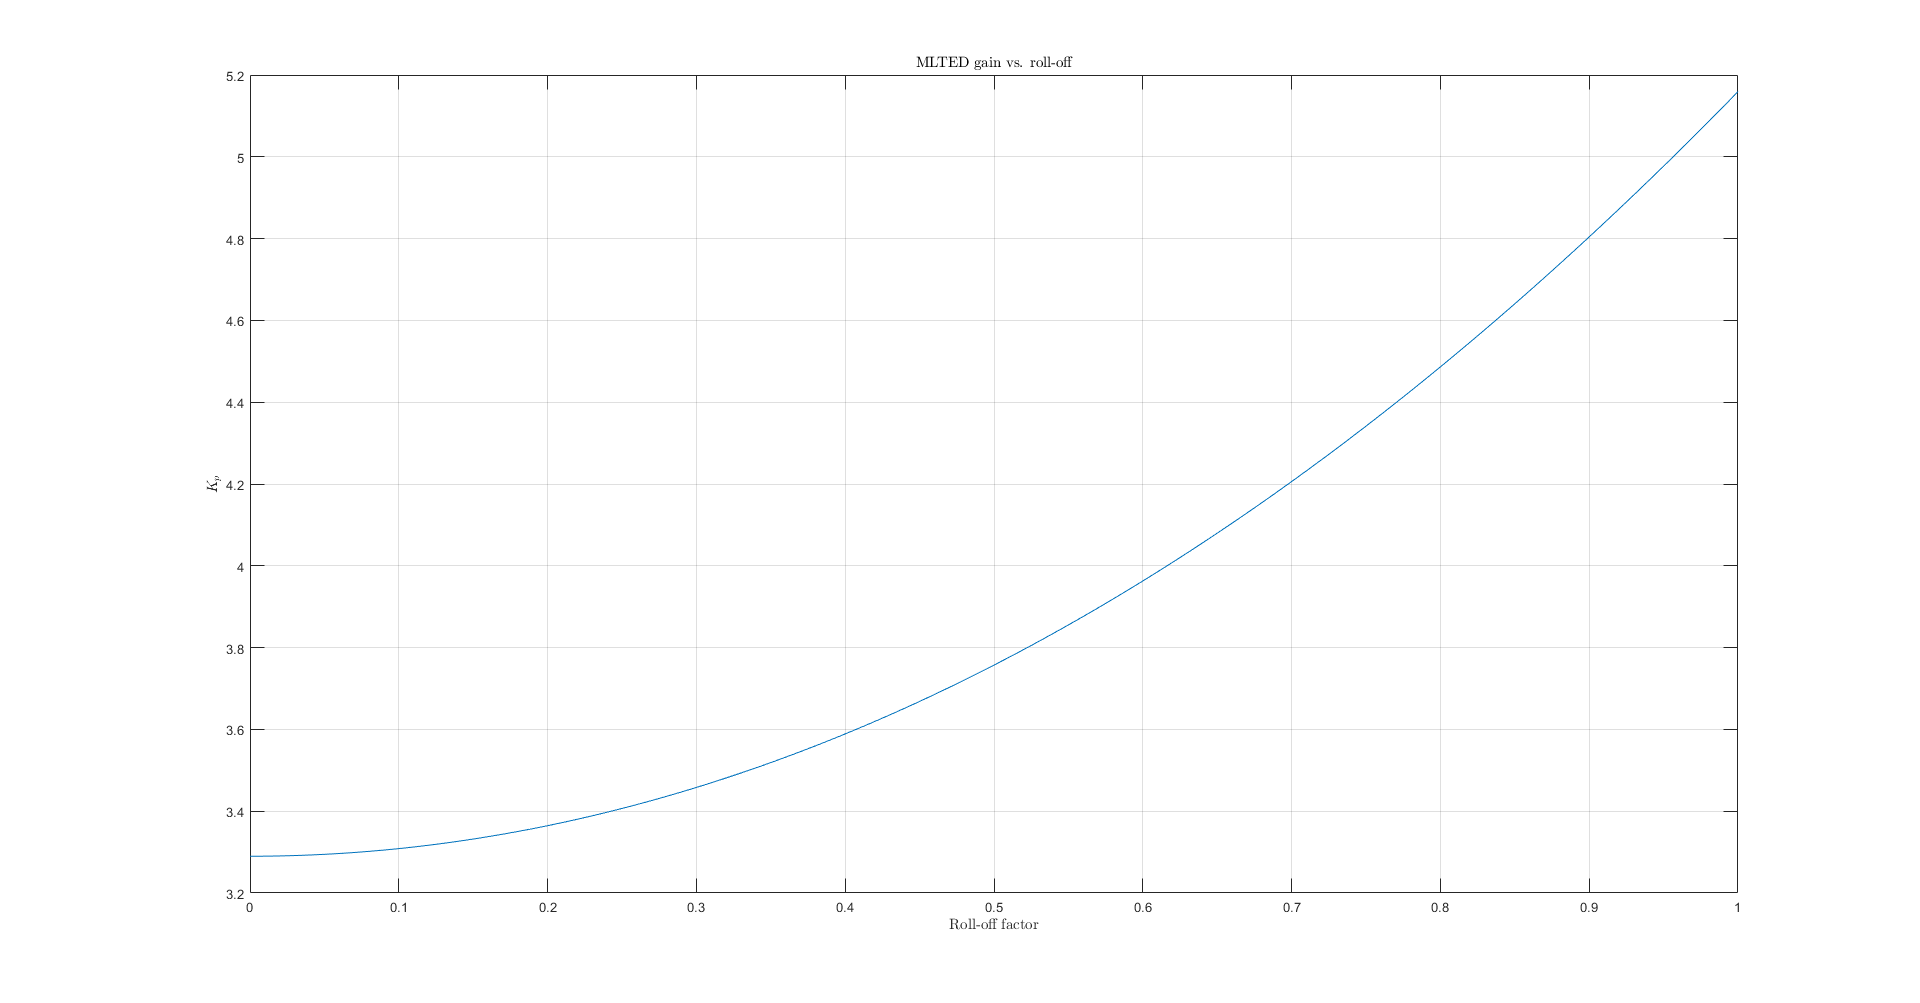
\includegraphics[width=0.85\linewidth]{img/intro/MLTEDgain.png}
    \caption{Evolução do \textit{TED Gain} face ao aumento do \textit{roll-off factor} (MLTED)\cite{igor}.} 
    \label{fig:TEDGain} 
\end{figure} 

O cálculo do ganho é dependente do \textit{roll-off factor} do \textit{root raised cosine} e do esquema do \textit{Timing Error Detector} utilizado (\textit{Maximum Likelihood}). Tal evolução é aparente na \hyperref[fig:TEDGain]{Fig. 5}. Para o \textit{roll-off factor} de $0.75$ especificado no Guia de Laboratório, o valor ótimo calculado\footnotemark[5] para o \textit{TED Gain} verificou-se $4.3415$. A aplicação deste fator é aparente na \hyperref[fig:TEDGain-effect]{Fig. 6}.

\footnotetext[5]{Através do cálculo analítico da constante, com o recurso ao \textit{script} em MATLAB disponibilizado em \href{https://github.com/igorauad/symbol_timing_sync}{https://github.com/igorauad/symbol\_timing\_sync}.}

\begin{figure}[ht]
    \centering
    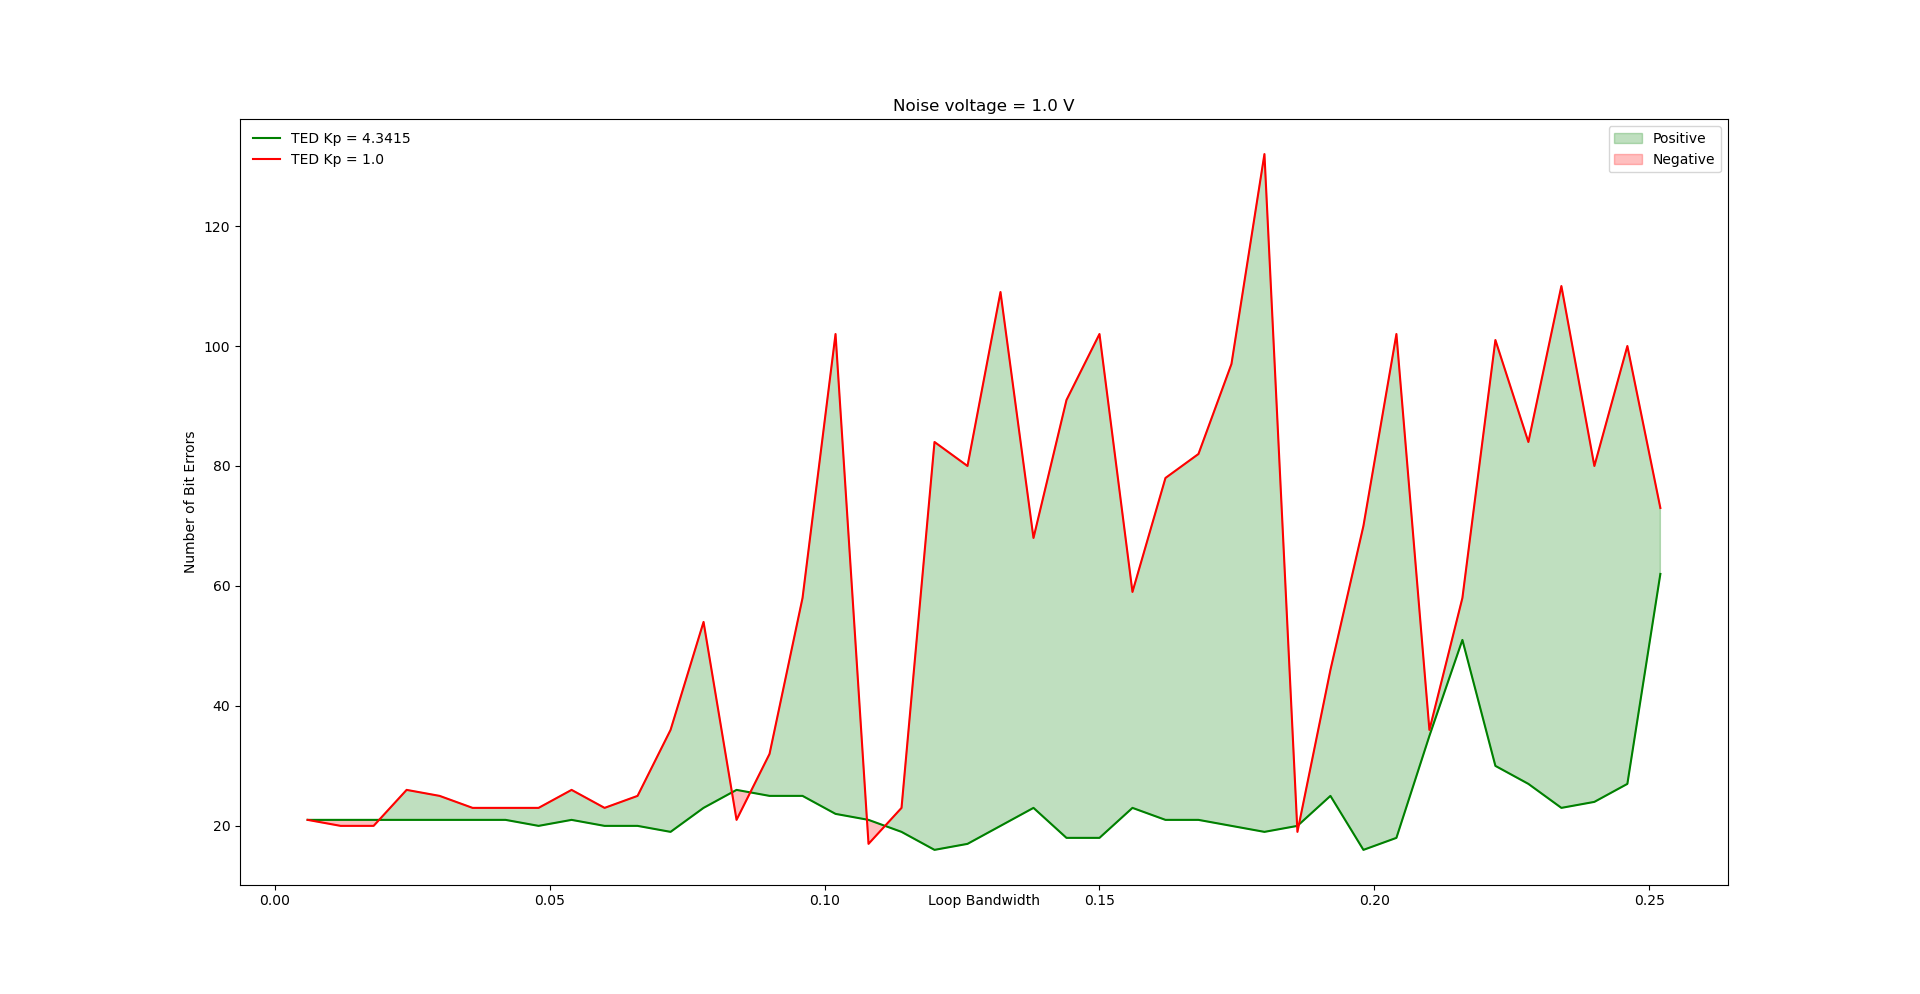
\includegraphics[width=0.85\linewidth]{img/intro/TEDGain_effect.png} 
    \caption{Efeitos da aplicação do \textit{TED Gain} calculado para uma \textit{noise voltage} de 1.0 V.} 
    \label{fig:TEDGain-effect} 
\end{figure} 

A maior estabilidade \hyperref[fig:TEDGain-effect]{observada} para o \textit{range} de valores de \textit{Loop Bandwidth} relevantes para a análise\cite{symbolsync-gnuradio}, é também acompanhada por uma desejável mitigação aparente de erros de bit\footnotemark[6]. Em virtude das ilações expostas, as posteriores simulações são, naturalmente, \textbf{realizadas com um \textit{TED Gain} de 4.3415}.

\footnotetext[6]{Reparos especialmente prevalentes para \textit{Loop Bandwidths} nominalmente perto de zero.}

\clearpage
\paragraph{3.1.2 \textit{Loop Bandwidth}}\mbox{}\\
A função do \textit{Loop Filter} encontrado na composição do bloco \textit{Symbol Sync} (\href{https://wiki.gnuradio.org/index.php/Symbol_Sync}{vide a documentação oficial}) pode ser sucintamente descrita pela seguinte citação:
\begin{quote}
    "\textbf{The loop filter controls how fast the timing error can be corrected, what types of errors can be treated, and the range of correctable timing errors.} In general, it is a second-order system and often the proportional-plus-integral controller (PI controller), commonly used in feedback systems. (...)"\cite{igor}
\end{quote}

O funcionamento deste integrante do processo de sincronizaç\~ao de símbolo é profundamente caracterizado pela sua \textit{Loop Bandwidth}, que:

\begin{quote}
    "(...) sets the boundary at which your recovery loop will track timing noise (jitter/phase noise) in your signal. \textbf{Timing noise has components at all frequencies} (...), and the lower frequency components of the timing noise (...) will be tracked by the timing loop, and therefore suppressed. However the higher frequency components will not be tracked by the timing loop and therefore remain and contribute to noise as part of SNR. \textbf{The timing loop can be viewed as a high pass filter on the jitter/phase noise components}, passing the higher frequency components (including the modulation signals) and supressing the lower frequencies at a rate depending on the order of the loop. Thus you see the motivation to make the timing loop as fast as possible in the interest of tracking out as much timing jitter as possible. \textbf{However, some of the signal energy of interest will be part of the "noise" being supressed by the timing loop}; and this can be quantified by understanding the spectral characteristics of the modulation used. \textbf{As the loop BW increases, too much signal energy is also removed}, and thus it is clear how there can be an optimum setting for the Loop BW that maximizes SNR."\cite{avi1987}
\end{quote}

Procuramos ent\~ao um valor de \textit{Loop Bandwidth} que n\~ao reduza (de forma comprometedora) a relaç\~ao sinal-ruído, mas que suprima as componentes de baixa e alta frequência do \textit{timing noise}. 

\vskip 1em
\noindent\fcolorbox{black}{white}{%
        \minipage[t]{\dimexpr\linewidth-2\fboxsep-2\fboxrule\relax}
            \textbf{Observação} $\rightarrow$ Em regime laboratorial, verifica-se geralmente o supracitado: o número de erros de bit tende\footnotemark[7] a aumentar consoante o incremento após certos \textit{thresholds} da \textit{Loop Bandwidth}, para cada patamar de ruído.
        \endminipage}

\footnotetext[7]{Relação aparente na análise posterior dos dois sistemas.}
%
%=============================--C--=============================%
\subsubsection{3.2 Reconversão para stream de dados binários}
\label{subsubsec:stream-to-bit}
Encontrado o intervalo ótimo de amostragem, ao qual corresponde o valor máximo do pulso, segue-se a conversão para \textit{stream} de dados binários, para a recuperação da sequência de \textit{bits} transmitida.

\clearpage
\paragraph{3.2.1 BPSK}\mbox{}\\
Para clarificar o processo corrente, é relevante apresentar um exemplo prático.

Observando a constelação do \textit{byte} 85 (0 1 0 1 0 1 0 1) repetido \textit{ad eternum}, na ausência dos efeitos do AWGN:
\begin{figure}[H]
    \begin{subfigure}[b]{0.45\linewidth}
        \centering
        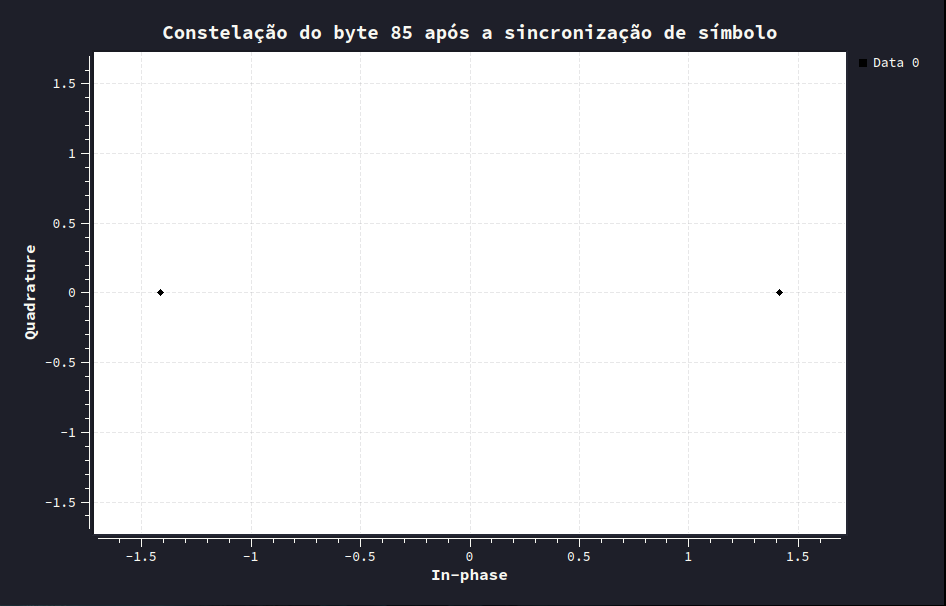
\includegraphics[width = 0.8\linewidth]{img/intro/const-byte85-bpsk.png}
        \caption{Constelação do \textit{byte} 85 após a sincronização\\ de símbolo.}
        \label{fig:const-byte85-bpsk}
        \vspace{1ex}
    \end{subfigure}
    \begin{subfigure}[b]{0.45\linewidth}
        \centering
        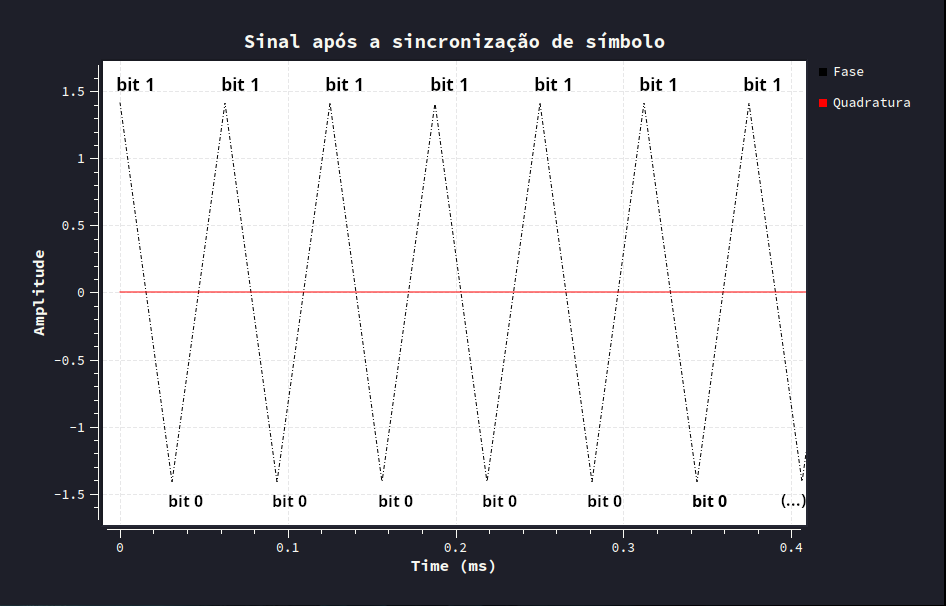
\includegraphics[width = 0.8\linewidth]{img/intro/detected-byte85-bpsk.png}
        \caption{Sinal correspondente ao \textit{byte} 85 após a sincronização de símbolo (sem presença de AWGN).}
        \label{fig:detected-byte85-bpsk}
        \vspace{1ex}
    \end{subfigure}
    \caption{Representações do \textit{byte} 85 numa modulação BPSK (sem normalização\protect\footnotemark[8]).}
\end{figure}
é aparente o mapeamento explicitado na antecedente \hyperref[subsubsec:const-mod]{secção 1.1}:
\vskip -2.5em
\begin{table}[H]
    \centering
    \begin{tabular}{c c}
        \minipage[t]{0.45\linewidth-2\fboxsep-2\fboxrule\relax}
            $$\text{\textit{bit}}\ 1 \mapsto [+1+0j] \xrightarrow[]{} \begin{cases}
                    \text{coef}_{\mathbb{R}\text{e}} = +\sqrt{2}\\
                    \text{coef}_{\mathbb{I}\text{m}} = 0
                \end{cases}
            $$
        \endminipage &\
        \minipage[t]{0.45\linewidth-2\fboxsep-2\fboxrule\relax}
            $$\text{\textit{bit}}\ 0 \mapsto [-1+0j] \xrightarrow[]{} \begin{cases}
                    \text{coef}_{\mathbb{R}\text{e}} = -\sqrt{2}\\
                    \text{coef}_{\mathbb{I}\text{m}} = 0
                \end{cases}
            $$
        \endminipage 
    \end{tabular}
\end{table}

Após a sincronização de símbolo (vide a \hyperref[fig:detected-byte85-bpsk]{Fig. 7} (b)), é apenas necessário recorrer a um bloco decisor para a conversão em \textit{bits} (\textit{Binary Slicer} $\xrightarrow[]{}$ "Positive input produces a binary 1 and negative input produces a binary zero."\cite{binaryslicer-gnuradio}) e efetuar um posterior agrupamento em \textit{bytes} (\textit{Pack K bits}). Tal como apresentado abaixo:

\begin{figure}[H]
    \centering
    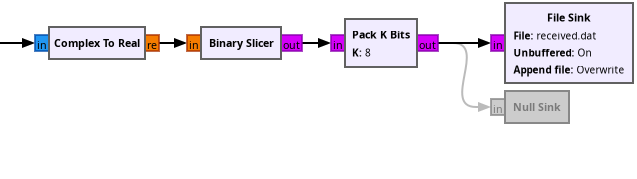
\includegraphics[width = 0.65\linewidth]{img/intro/BPSK_demod.png}
    \caption{Etapa final do processo de desmodulação BPSK em ambiente \textit{GNU Radio}.}
    \label{fig:bpsk-demod}
\end{figure}

\noindent\fcolorbox{black}{white}{%
        \minipage[t]{\dimexpr\linewidth-2\fboxsep-2\fboxrule\relax}
            \textbf{Observação} $\rightarrow$ Em regime laboratorial, verifica-se um \textit{offset} de 49 \textit{bits} no ficheiro ‘received.dat' (ficheiro de saída, vide a \hyperref[fig:bpsk-demod]{Fig. 8}), tal como explicitado no Guia de Laboratório: "(...) De notar que no ficheiro ‘bpsk\_rec.dat', os bits correspondentes aos bits enviados aparecem a partir da 50\textsuperscript{\underline{a}} posição sendo precedidos de 49 bits correspondentes ao buffer interno do módulo ‘Symbol Sync’"\cite{guia_lab}.
        \endminipage}

\footnotetext[8]{Devido a incongruências observadas em diversas plataformas (Windows, GNU/Linux) da opção \textit{Normalization Type} do bloco \hyperref[subsubsec:const-mod]{\textit{Constellation Object}} \cite{constellationobject-gnuradio} em ambiente \textit{GNU Radio}, \textbf{toda a análise subsequente é realizada sem qualquer tipo de normalização} (i.e., $\sqrt{\varepsilon} = \sqrt{2} \neq 1$), de modo a garantir a comparação dos sistemas BPSK e QPSK.}

%---
\clearpage
\paragraph{3.2.2 QPSK}\mbox{}\\
De forma análoga, apresenta-se o exemplo do \textit{byte} 153 (10 01 10 01), em repetição, que nos permite observar a sincronia ortogonal das componentes em fase e em quadratura (característica da modulação QPSK\footnotemark[9]).

\footnotetext[9]{"QPSK can be regarded as a pair of orthogonal BPSK systems, i.e. the real component is one BPSK system, the imaginary component is the second BPSK 
system (...)"\cite{dsp}}

\begin{figure}[H]
    \begin{subfigure}[b]{0.45\linewidth}
        \centering
        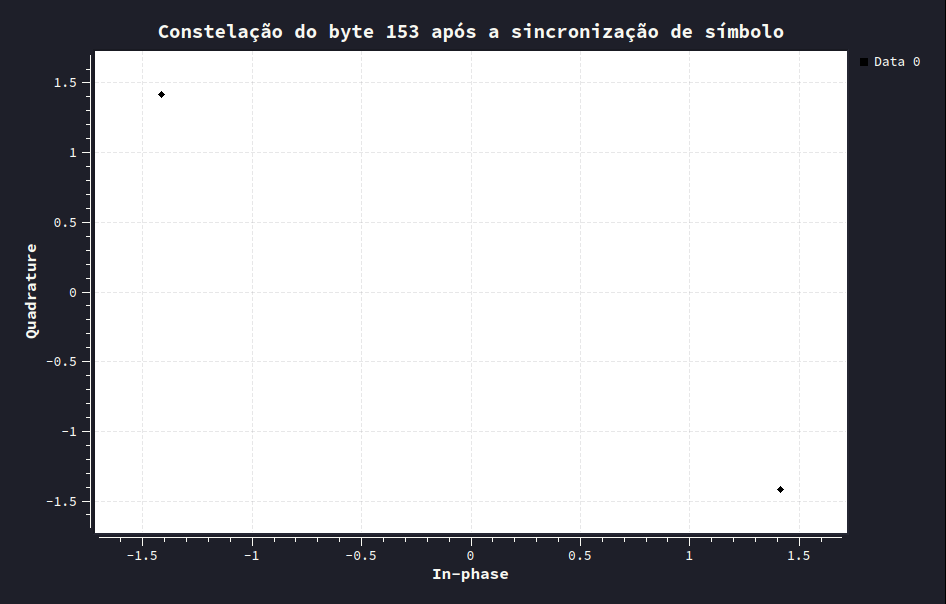
\includegraphics[width = 0.8\linewidth]{img/intro/const-byte153-qpsk.png}
        \caption{Constelação do \textit{byte} 153 após a sincronização\\ de símbolo.}
        \label{fig:const-byte153-qpsk}
        \vspace{1ex}
    \end{subfigure}
    \begin{subfigure}[b]{0.45\linewidth}
        \centering
        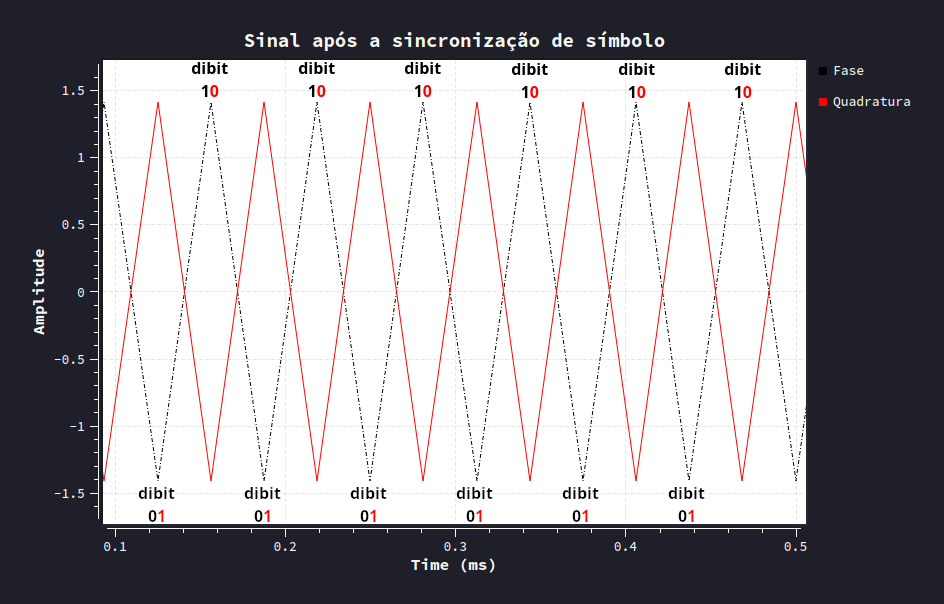
\includegraphics[width = 0.8\linewidth]{img/intro/detected-byte153-qpsk.png}
        \caption{Sinal correspondente ao \textit{byte} 153 após a sincronização de símbolo (sem presença de AWGN).}
        \label{fig:detected-byte153-qpsk}
        \vspace{1ex}
    \end{subfigure}
    \caption{Representações do \textit{byte} 153 numa modulação QPSK (sem normalização).}
\end{figure}
Ainda assim, graças à particularidade referida acima (e na anterior \hyperref[subsubsec:const-mod]{secção 1.1}), um \textit{byte} seccionado em \textit{dibits} pode ser mapeado (de forma ótima, sem AWGN) para as quatro regiões do diagrama de constelação, como se apresenta:

\vskip -2.5em
\begin{table}[h]
    \centering
    \begin{tabular}{l l}
        \minipage[t]{0.5\linewidth-2\fboxsep-2\fboxrule\relax}
            $$
            \begin{tabular}{c}
                \textit{dibit}\\
                11
                \end{tabular} \mkern-9mu\mapsto [+1+1j] \xrightarrow[]{} \begin{cases}
                    \text{coef}_{\mathbb{R}\text{e}} = +\sqrt{2}/2\\
                    \text{coef}_{\mathbb{I}\text{m}} = +\sqrt{2}/2
                \end{cases}
            $$
        \endminipage &\
        \minipage[t]{0.5\linewidth-2\fboxsep-2\fboxrule\relax}
            $$
            \begin{tabular}{c}
                \textit{dibit}\\
                01
                \end{tabular} \mkern-9mu\mapsto [-1+1j] \xrightarrow[]{} \begin{cases}
                    \text{coef}_{\mathbb{R}\text{e}} = -\sqrt{2}/2\\
                    \text{coef}_{\mathbb{I}\text{m}} = +\sqrt{2}/2
                \end{cases}
            $$
        \endminipage \\ 
        \minipage[t]{0.5\linewidth-2\fboxsep-2\fboxrule\relax}
            $$
            \begin{tabular}{c}
                \textit{dibit}\\
                00
                \end{tabular} \mkern-9mu\mapsto [-1-1j] \xrightarrow[]{} \begin{cases}
                    \text{coef}_{\mathbb{R}\text{e}} = -\sqrt{2}/2\\
                    \text{coef}_{\mathbb{I}\text{m}} = -\sqrt{2}/2
                \end{cases}
            $$
        \endminipage &\ 
        \minipage[t]{0.5\linewidth-2\fboxsep-2\fboxrule\relax}
            $$
            \begin{tabular}{c}
                \textit{dibit}\\
                10
                \end{tabular} \mkern-9mu\mapsto [+1-1j] \xrightarrow[]{} \begin{cases}
                    \text{coef}_{\mathbb{R}\text{e}} = +\sqrt{2}/2\\
                    \text{coef}_{\mathbb{I}\text{m}} = -\sqrt{2}/2
                \end{cases}
            $$
        \endminipage
    \end{tabular}
\end{table}

Novamente, após este processo de deteção, segue-se a conversão para \textit{stream} de dados binários, empacotados posteriormente em \textit{bytes}. Este processo assemelha-se ao do BPSK, com a exceção da intercalação das componentes em fase (\textit{bit} mais significativo do \textit{dibit}) e em quadratura (\textit{bit} menos significativo do \textit{dibit}).  

\begin{figure}[H]
    \centering
    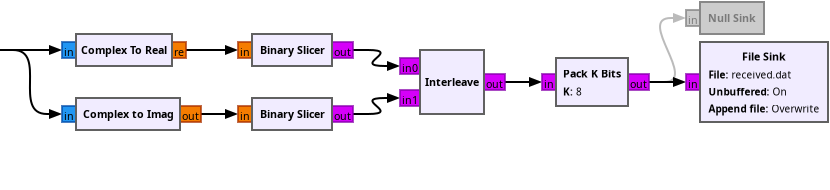
\includegraphics[width = 0.85\linewidth]{img/intro/QPSK_demod.png}
    \caption{Etapa final do processo de desmodulação QPSK em ambiente \textit{GNU Radio}.}
    \label{fig:qpsk-demod}
\end{figure}

\noindent\fcolorbox{black}{white}{%
        \minipage[t]{\dimexpr\linewidth-2\fboxsep-2\fboxrule\relax}
            \textbf{Nota} $\rightarrow$ Verifica-se uma duplicação do \textit{offset} (proveniente do \textit{buffer} do \textit{Symbol Sync}) incutido no ficheiro de saída, (fenómeno esperado) visto que decorrem duas sincronizações em paralelo\footnotemark[9] posteriormente intercaladas. 
        \endminipage}